\subsection{2.2 Orbitals}
  \begin{minipage}{0.99\linewidth}
    \begin{minipage}{0.33\linewidth}
      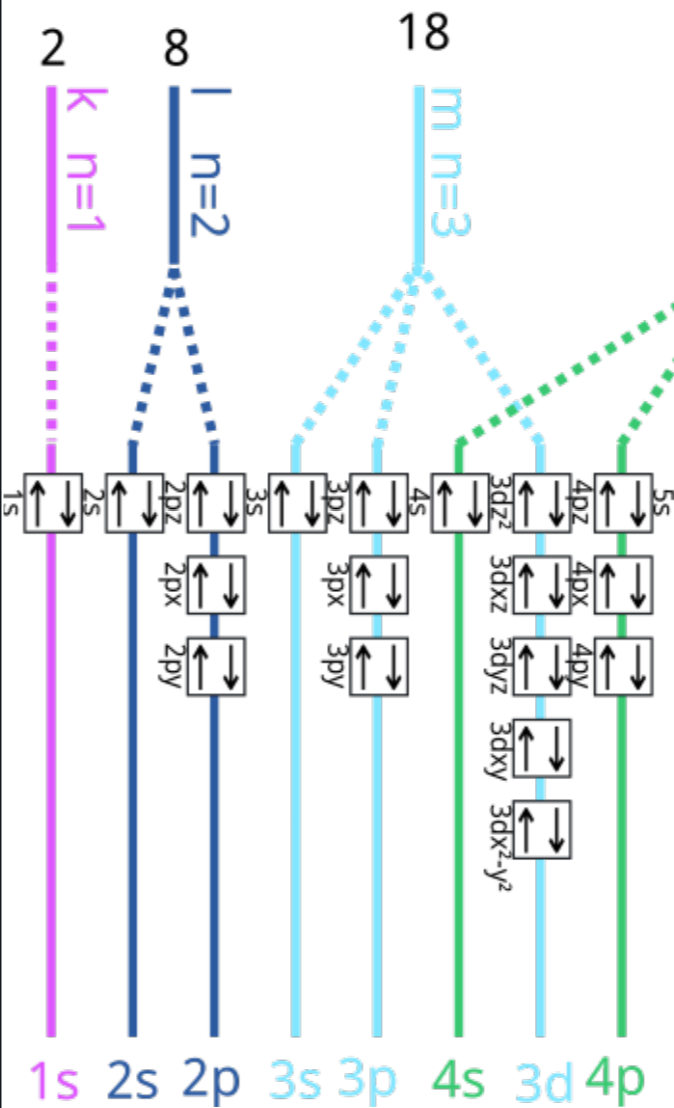
\includegraphics[width = 2.3cm]{src/2_Atoms/images/Energieniveau.png}
    \end{minipage}
    \begin{minipage}{0.52\linewidth}
      \begin{scriptsize}
        \begin{center}
            \begin{tabular}{|p{0.3mm}|c|p{0.07\textwidth}|c|c|}
                \multicolumn{1}{p{0.3mm}}{n} & \multicolumn{1}{c}{l} & \multicolumn{1}{p{0.07\textwidth}}{\rotatebox{90}{\pbox{1.5cm}{subshell\\ designation}}} & \multicolumn{1}{c}{$m_i$} & \multicolumn{1}{c}{$m_s$} \\ [0.5ex]
                \hline
                1 & 0, s & 1s                                  & 0                      & $\pm 1/2$ \\ 
                \hline
                2 & 0, s & 2s                                  & 0                      & $\pm 1/2$ \\
                  & 1, p & 2p                                  & 1, 0, -1               & $\pm 1/2$ \\
                \hline
                3 & 0, s & 3s                                  & 0                      & $\pm 1/2$ \\
                  & 1, p & 3p                                  & 1, 0, -1               & $\pm 1/2$ \\
                  & 2, d & 3d                                  & 2, 1, 0, -1, -2        & $\pm 1/2$ \\
                \hline
                4 & 0, s & 4s                                  & 0                      & $\pm 1/2$ \\
                  & 1, p & 4p                                  & 1, 0, -1               & $\pm 1/2$ \\
                  & 2, d & 4d                                  & 2, 1, 0, -1, -2        & $\pm 1/2$ \\
                  & 3, f & 4f                                  & 3, 2, 1, 0, -1, -2, -3 & $\pm 1/2$ \\
                \hline
            \end{tabular}
        \end{center}
        \end{scriptsize}
    \end{minipage}
  \end{minipage}
        
    \begin{itemize}
        \itemsep0em
        \item \textbf{n}: principal quantum number $\rightarrow$ size of orbital
        \item \textbf{l}: angular quantum number $\rightarrow$ shape of orbital
        \item $\boldsymbol{m_l}$: magnetic quantum number $\rightarrow$ orientation of orbital
        \item $\boldsymbol{m_s}$: spin quantum number
    \end{itemize}
    \vspace*{-0.9em}
    
    \begin{minipage}{0.99\linewidth}
      \begin{minipage}{0.45\linewidth}
        \centerline{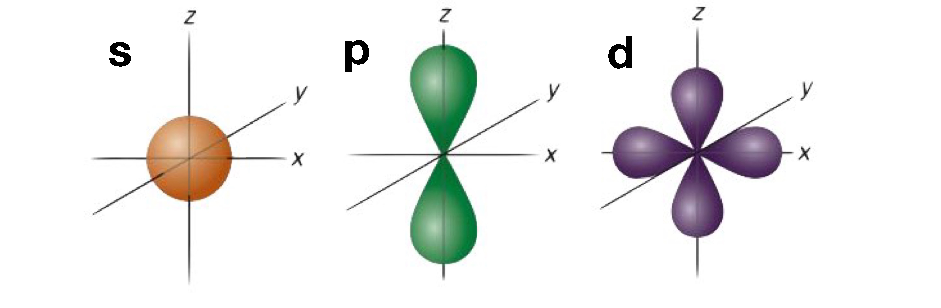
\includegraphics[width=35mm]{src/2_Atoms/images/orbital_shapes.pdf}}
      \end{minipage}
      \begin{minipage}{0.54\linewidth}
        \centerline{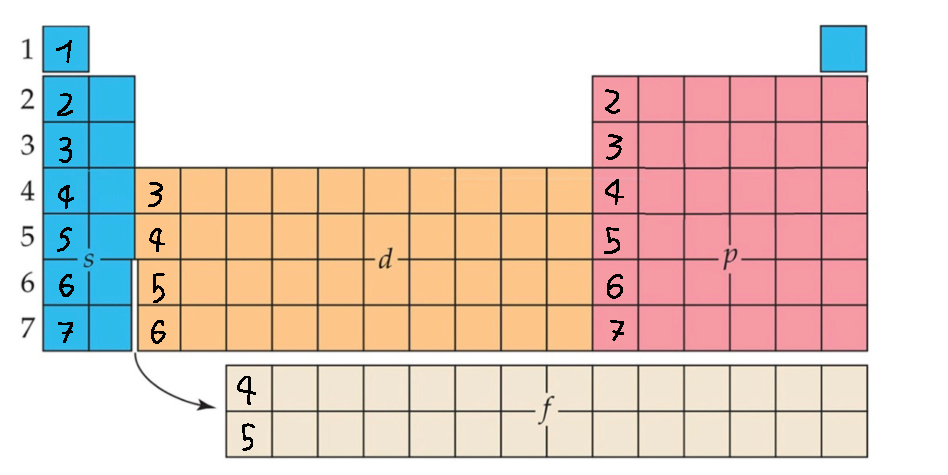
\includegraphics[width=43mm]{src/2_Atoms/images/pse_electron_config.pdf}}
      \end{minipage}
    \end{minipage}
    
    Pauli Exclusion: Each electron has unique set of quantum numbers\\
    Hund's rule: \textbf{Every} orbital in sublevel is first singly occupied\\
    Energy of Hydrogen $e^-$: $E_n = -\frac{hcR_H}{n^2}$, $R_h = 1.097 \cdot 10^7 m^{-1}$\\
    Excitement from shell $n_1$ to $n_2$: $E_H = hcR_H (\frac{1}{n_1^2} - \frac{1}{n_2^2})$